\chapter{The ORBM: A model of independent complex causes}

\section{A network equivalent to an RBM}

\subsection{Unrolling a Gibbs Chain, a different perspective on RBM inference}

\begin{wrapfigure}{r}{0.6\textwidth}
  \begin{center}
    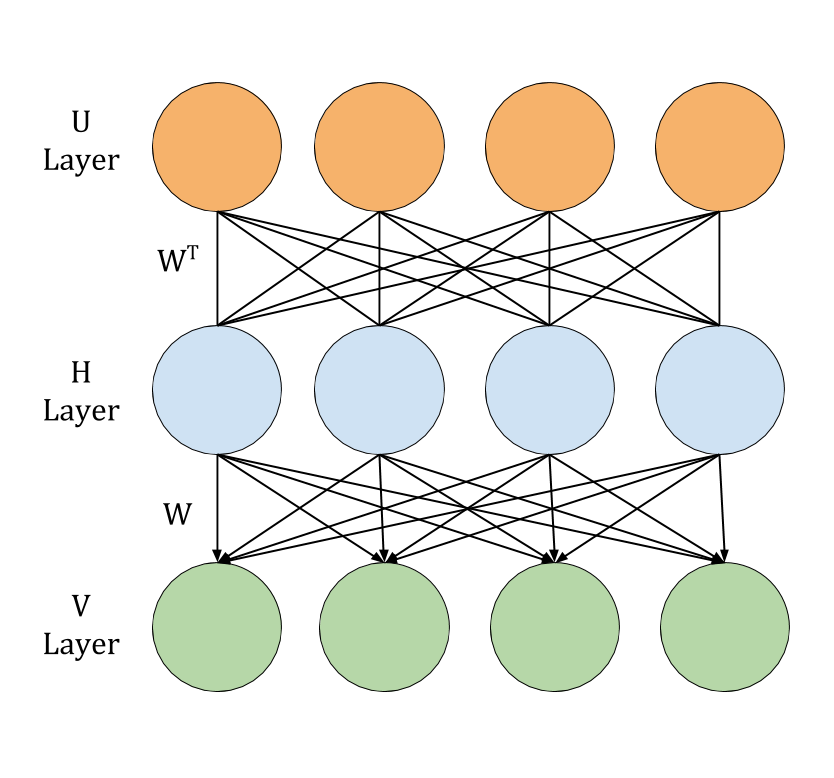
\includegraphics[width=0.5\textwidth]{Assets/3_Layer_RBM.png}
  \end{center}
  \caption{A diagram illustrating `unrolling` an RBM by one Gibbs iteration. Note the connections between $H$ and $V$ layers are now directed.}
  \label{F:3-Layer-RBM}
\end{wrapfigure}

Before the ORBMs architecture and inference algorithm can be introduced, Gibbs sampling in an RBM must be presented in a different, yet equivalent way.
Hinton, when introducing the idea of training a Deep Belief Network showed that a Gibbs chain in an RBM is equivalent to a infinitely deep belief network, with an RBM on the top with tied weights. \todocite{Hintons paper on unrolling the Gibbs chain}. An unrolling of a single Gibbs iteration is illustrated in figure \ref{F:3-Layer-RBM}, the $U$ layer corresponding to the $V$ layer after one Gibbs iteration. The top two layers ($U$ and $H$) form a standard RBM, but the bottom connections ($V$ and $H$) form a Sigmoid Belief Network. To further clarify, the $U$ layer corresponds to $V_1$ in figure \ref{F:Gibbs_Chain}. Note in figure \ref{F:3-Layer-RBM} the weights  between the $H$ and $U$ layer are shared between the $V$ and $H$ layers.

We can now show that Gibbs sampling in this RBM unrolled with a Sigmoid belief network is equivalent to Gibbs Sampling in a standard RBM.\@

\subsubsection{Sampling in this equivalent network}

sampling in the ORBM \todocite{as described in the section where I talk about dreams...} network behaves a similar way to RBM sampling, where a Gibbs chain is run between the top two layers, $U$ and $H$, until the last iteration. At the last iteration a hidden pattern is sampled and then is pushed through the Sigmoid belief network between $H$ and $V$. This is illustrated in figure \ref{F:3-Layer-RBM-Gibbs}.

\begin{figure}[h]
\begin{center}
  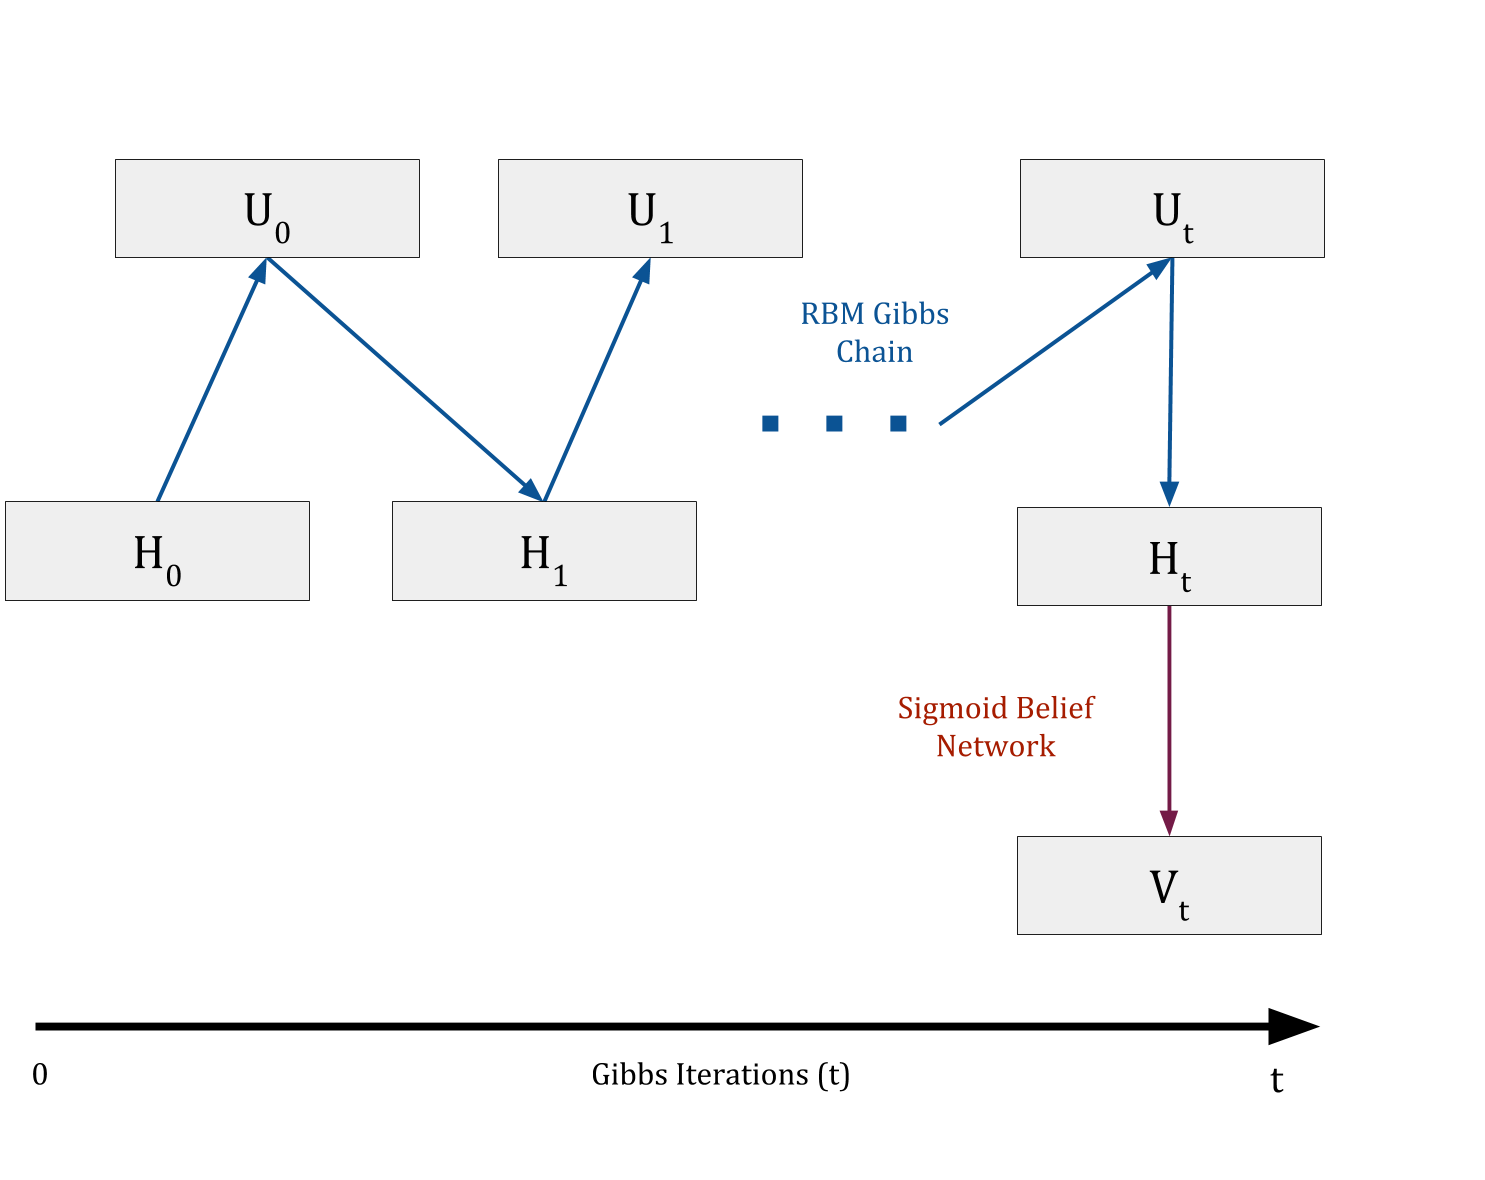
\includegraphics[width = 0.8\textwidth]{Assets/ORBM-Gibbs-Chain.png}
\caption{A diagram showing Ancestral sampling in the equivalent network, where normal sampling in the top 2 layers is performed until Gibbs iteration $t$ the hidden state is pushed through the bottom layers Sigmoid Network.}
\label{F:3-Layer-RBM-Gibbs}
\end{center}
\end{figure}

To generate a sample from $h$ is equivalent we can use equation \ref{eq:Hid-Gibbs-Update}, by running the Gibbs chain between $h$ and $U$. To sample from $v$ in the SBN is by definition:
$$
P(v_i = 1|h) = \sigma_i(h)
$$
Thus Gibbs sampling from a simple RBM ending in a sample for $v$ is the same as sampling $h$ from the same RBM and using a SBN for the last step.

There is however another useful way to draw samples in such a network that we will leverage in the ORBM. The log likelihood of the joint can be written as:
\begin{equation}\label{eq:Product-Joint}
\log P^\star(h,v) = \log P^\star(h) + \log P(v|h)
\end{equation}
The second term is defined in equation \ref{eq:SBN-v-given-h}. To find the first term, $P^\star(h)$, we need to marginalise the joint (eq~\ref{eq:Product-Joint}) over all $\mathbf{U}$ layer configurations:

$$
 \begin{aligned}
P^\star(h) &= \sum_{v_1=0}^1 \cdots \sum_{v_n=0}^1 \exp \bigg[  \log P^{\star}(h,v) \bigg] \\
&= \sum_{v_1=0}^1 \cdots \sum_{v_n=0}^1 \exp \bigg[  \sum_i  \sum_j h_j W_{ji} v_i \;\; + \;\; \sum_i W_{0i} v_i \;\; + \;\; \sum_j W_{j0} h_j \bigg] \\
&= \sum_{v_1=0}^1 \cdots \sum_{v_n=0}^1 \exp \bigg[  \sum_i v_i \phi_i(h)  \;\; + \;\; \sum_j W_{j0} h_j \bigg] \\
&= \exp\left[ \sum_j h_j  W_{j0} \right] \;\; \times \sum_{v_1=0}^1 \cdots \sum_{v_n=0}^1 \prod_i \exp\bigg[ v_i \phi_i(h) \bigg] \\
&= \exp\left[\sum_j h_j  W_{j0}\right] \;\; \times \prod_i \bigg( 1 + e^{\phi_i(h) } \bigg) \\
\text{and taking logs,}
\log P^\star(h) &= \sum_j h_j  W_{j0} \;\; +  \sum_i \log \bigg( 1 + e^{\phi_i(h) } \bigg)
\\
&= \sum_j h_j  W_{j0} \;\; + \; \sum_i \phi_i(h) \;  - \; \sum_i \log \sigma_i(h)
\end{aligned}
$$

So far we've figured out $\log P^\star(h)$ for the RBM that is the `top layer`.

Therefore another way to write $\log P^\star(h,v)$ is
\begin{equation}\label{eq:equivalent-rbm-log-joint}
\log P^\star(h,v) = \underbrace{\sum_j h_j  W_{j0} \;\; + \; \sum_i \phi_i(h) \;  - \; \sum_i \log \sigma_i(h)}_{\log P^\star(h)} \;\;+\;\; \underbrace{\sum_i v_i \log \sigma_i(h) + (1-v_i) \log (1 - \sigma_i(h))}_{\log P(v \mid h)}
\end{equation}
By collecting terms and simplifying this matches the earlier form in equation~\ref{eq:LogPJoint}.


\section{A New Approach, The ORBM}

\subsection{Architecture}

Frean and Marsland extend on this idea of a one Gibbs iteration unrolled RBM. They propose adding another $U$ and $H$ layers to represent another rich source of data, which then combines with the orignal $U$ and $H$ layer via a SBN to form $V$. This architecture is illustrated in figure \ref{ORBM-Architecture}, where A and B are used to denote the two independant causes we are modeling. To clarify the ORBMs architecture, there are two RBMs, one for each cause. These RBMs are connected to a SBN into the visible layer, the weights of which are tied to the respective RBMs. This architecture is simpler in practice as the U layers can be captured in the inference algorithm.

By building on RBMs and SBN we can leverage existing algorithms and work on RBMs and also the potential for extending this work to deeper architectures is possible. Also the architecture supports `plug and play` with the models in that existing RBMs can be plugged into the architecture. The implications of this are exciting in that an RBM that has been trained on hand written digits could be plugged into an RBM that has been trained on a paper texture (the bumps and ridges of paper). Then using the ORBM a `clean` representation of the text and paper could be separated out given an image of a digit on paper.

The ORBM, like the RBM is difficult to evaluate empirically, but the same techniques that can be used to evaluate RBMs can be applied to the ORBM.\@

\begin{figure}[h]
\begin{center}
  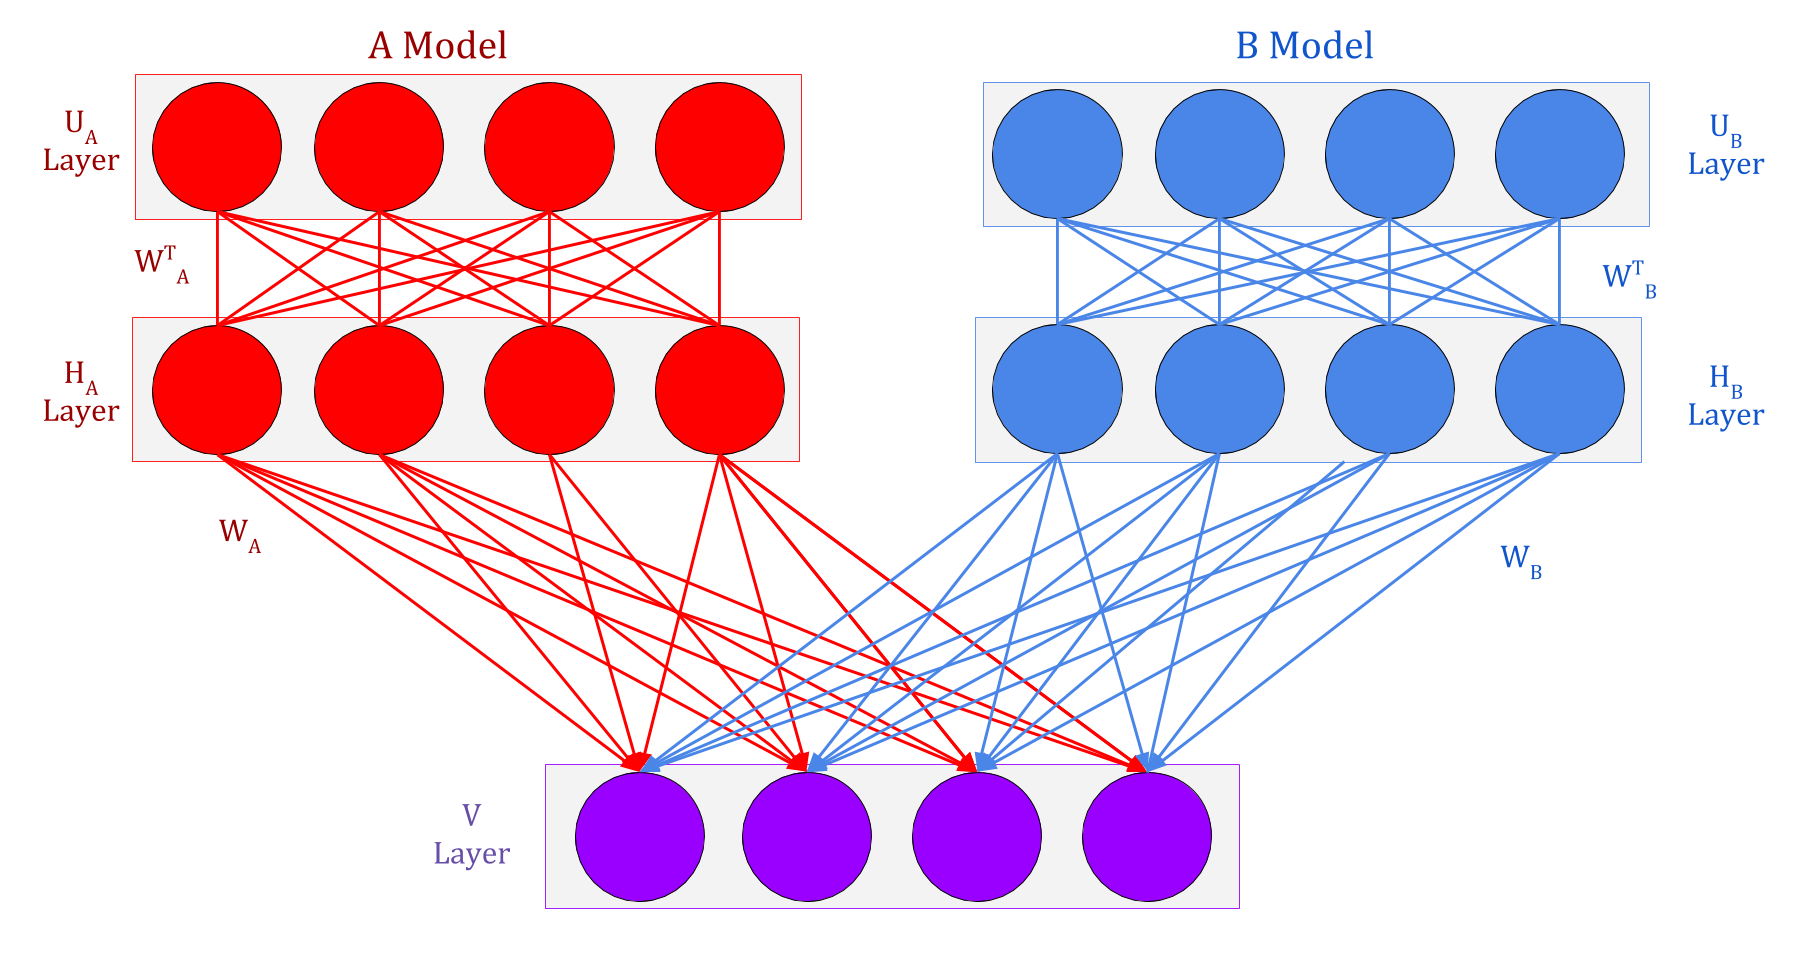
\includegraphics[width = 1.2\textwidth]{Assets/ORBM-Full-Architecture.png}
\caption{The full ORBM architecture, where $A$ and $B$ are the two causes that combine to form the data.}
\label{ORBM-Architecture}
\end{center}
\end{figure}

\subsection{Gibbs Sampling in the ORBM}

\subsubsection{Ancestral Sampling in the ORBM}

Ancestral sampling in an RBM involved running a Gibbs chain and then taking the last visible in that chain. To perform ancestral sampling in the ORBM we can leverage the generative power of the RBM and then combine their inputs in a simple way.
We know that joint in the unrolled RBM is expressed as eq~\ref{eq:Product-Joint}.
That is, the ORBM probability of $v$ given $h^{A} $ and $h^{B}$ is defined by:
$$ \log P(v|h^A,h^B) = \sum_i v_i \log \sigma (\phi^A_i + \phi^B_i) + (1-v_i) \log (1 - \sigma(\phi^A_i + \phi^B_i)$$
Where $\phi_i^A \text{ and } \phi_i^B $ are the weighted sums into the $ ith$ visible units from the models A and B respectively. In this generative model a visible unit is created by taking the weighted sum from both sources, adding their contribution and then passing through a Sigmoid function to give a probability.

\subsubsection{Inference in the ORBM}

In a standard RBM sampling from $P(h_j)$ is given by $P(h_j) = \sigma(\psi_i)$, where $\psi_i$ is defined in equation \ref{psi-gibbs-update-rbm}. In an ORBM we cannot consider the single RBM alone when trying to find $P(h_j)$, as the hidden layers of the two RBMs in the ORBM are dependent given a visible layer $v$. This amounts to explaining away as described in section \ref{SS:Explaining-Away}. There is a nice feature of the ORBM in that the hidden representations ($ h^A \text{ and } h^B $) we extract from the visible layer require no interaction with the $U$ layers to sample from. They are only needed to generate a composite $V$ pattern (or independent reconstructions).

We aim to use Gibbs sampling to generate $ h^A \text{ and } h^B $ given a $ v $:
We need to calculate
$$
\psi^A_j = \log P^\star(h,v | h^A_j = 1) - \log P^\star (h,v| h^A_j = 0)
$$
We will use that fact that the weighted sum into a visible unit $i$ where some hidden unit $h_j$ is on, is equivalent to the same configuration except $h_j$ is off plus the weight between these two units. This is by definition true, and expressed below:
$$
\phi^A_i(h | h^A_j=1) = \phi^A_i(h | h^A_j=0) + W^A_{ji}
$$
We will abbreviate $\phi^A_i(h | h_j=0)$ to $\phi^{Aj0}_i$. Given these we obtain:
$$
\psi^A_j = \sum_i v_i \log \left( \frac{1+ e^{-\phi^{Aj0}_i - \phi^B_i}}{1+e^{-\phi^{Aj0}_i - W_{ji} -\phi^B_i}} \frac{1+ e^{\phi^{Aj0}_i + W_{ji} + \phi^B_i}}{1+e^{\phi_i^{Aj0} + \phi^B_i}}\right) \;\;+ \;\;\sum_i \log \left(\frac{1+e^{\phi_i^{Aj0} + W_{ji}}}{1+ e^{\phi_i^{Aj0}}}
\frac{1+e^{\phi_i^{Aj0} + \phi^B_i}}{1+ e^{\phi_i^{Aj0} + W_{ji} + \phi^B_i}} \right)
$$

Now $\phi = \log \frac{1+e^{\phi}}{1+e^{-\phi}}$ (Marcus' magic identity), which is$ = \log \frac{\sigma(\phi)}{\sigma(-\phi)}$.
So the first term simplifies to
$ \sum_i v_i W_{ji}$, which is the same as that in an RBM. The second term can also be simplified, using the identity $\log(1-\sigma(\phi)) = \phi - \log(1+e^\phi)$. This leads to the following Gibbs Sampler probability of the j-th hidden unit in network $A$ being 1: $p_j = \sigma(\psi_j^A)$ with

$$
\psi_j^A = \underbrace{\sum_i W^A_{ji} v_i}_\text{vanilla RBM} \; + \; \underbrace{\sum_i C^A_{ji}}_\text{correction} $$
where the correction is:
\begin{equation}\label{eq:Full-Corretion}
\begin{aligned}
C^A_{ji} \; &= \;\log \bigg[ \frac{\sigma (\phi_i^{Aj0})}{\sigma (\phi_i^{Aj0} + W^A_{ji})} . \frac{\sigma (\phi_i^{Aj0} + W_{ji}^A + \phi_i^B) }{\sigma (\phi_i^{Aj0} + \phi_i^B)} \bigg]
\\
&= \log \sigma(\phi_i^{Aj0})  \; + \; \log \sigma (\phi_i^{Aj0} + W^A_{ji} + \phi_i^B) \;- \log \sigma (\phi_i^{Aj0} + W^A_{ji})  \; - \; \log \sigma ( \phi_i^{Aj0} + \phi_i^B)
\\
&= \log \bigg[ \frac{\sigma(\phi_i^{A} - h^A_i W^A_{ji})}{\sigma (\phi_i^{A} + (1-h^A_i) W^A_{ji})} \bigg]  \; - \; \log \bigg[ \frac{ \sigma ( \phi_i^{AB} - h^A_i W^A_{ji})}{\sigma (\phi_i^{AB} + (1-h^A_i) W^A_{ji})} \bigg]
\end{aligned}
\end{equation}
where $\phi_i^{AB} = \phi_i^{A} + \phi_i^{B}$. Note that $v$ plays no role in the correction. It is clear that adding $\phi^B_i$ has introduced a dependency between the entirety of $h$. This means that a Gibbs chain will need to be run, in practice this chain proves to be short, even in the larger dimension tasks like MNIST.

\subsubsection{Examining and approximating the Correction}

This correction (eq \ref{eq:Full-Corretion}) is a non-trivial computation to make in that for every weight, a series of semi-large matrix operations have to be performed. As a result, Frean and Marsland propose an approximation for this correction.

It is useful to see the correction contours on axes $\phi^A_i$ versus $\phi^{AB}_i$, for a positive weight $W^A_{ij}$.
There are two plots for the two cases $h^A_j=0,1$ These are plotted in figure \ref{F:Correction-Plot}. From these plots we can see that this function has defined `plataus` where the height of these platuas is $+_-$ the weight respectively. The correction essentailly adjusts the weight between $v_i$ and $h_j$ allowing it to be turned off, turned on, intensified, deintensified, or have no effect. This is similar to adjusting the visible activation based on what the two RBMs are doing and hence Frean and Marsland propose the following approximation:

\begin{equation}\label{eq:Approx-Correction}
 C^A_{ji} = \sigma(\phi^{A_{j0}}_i + W^A_{ji}) - \sigma(\phi^{A_j0}_i W^A_{ji} + \phi^B_i)
\end{equation}


\begin{figure}[h]
\begin{center}
  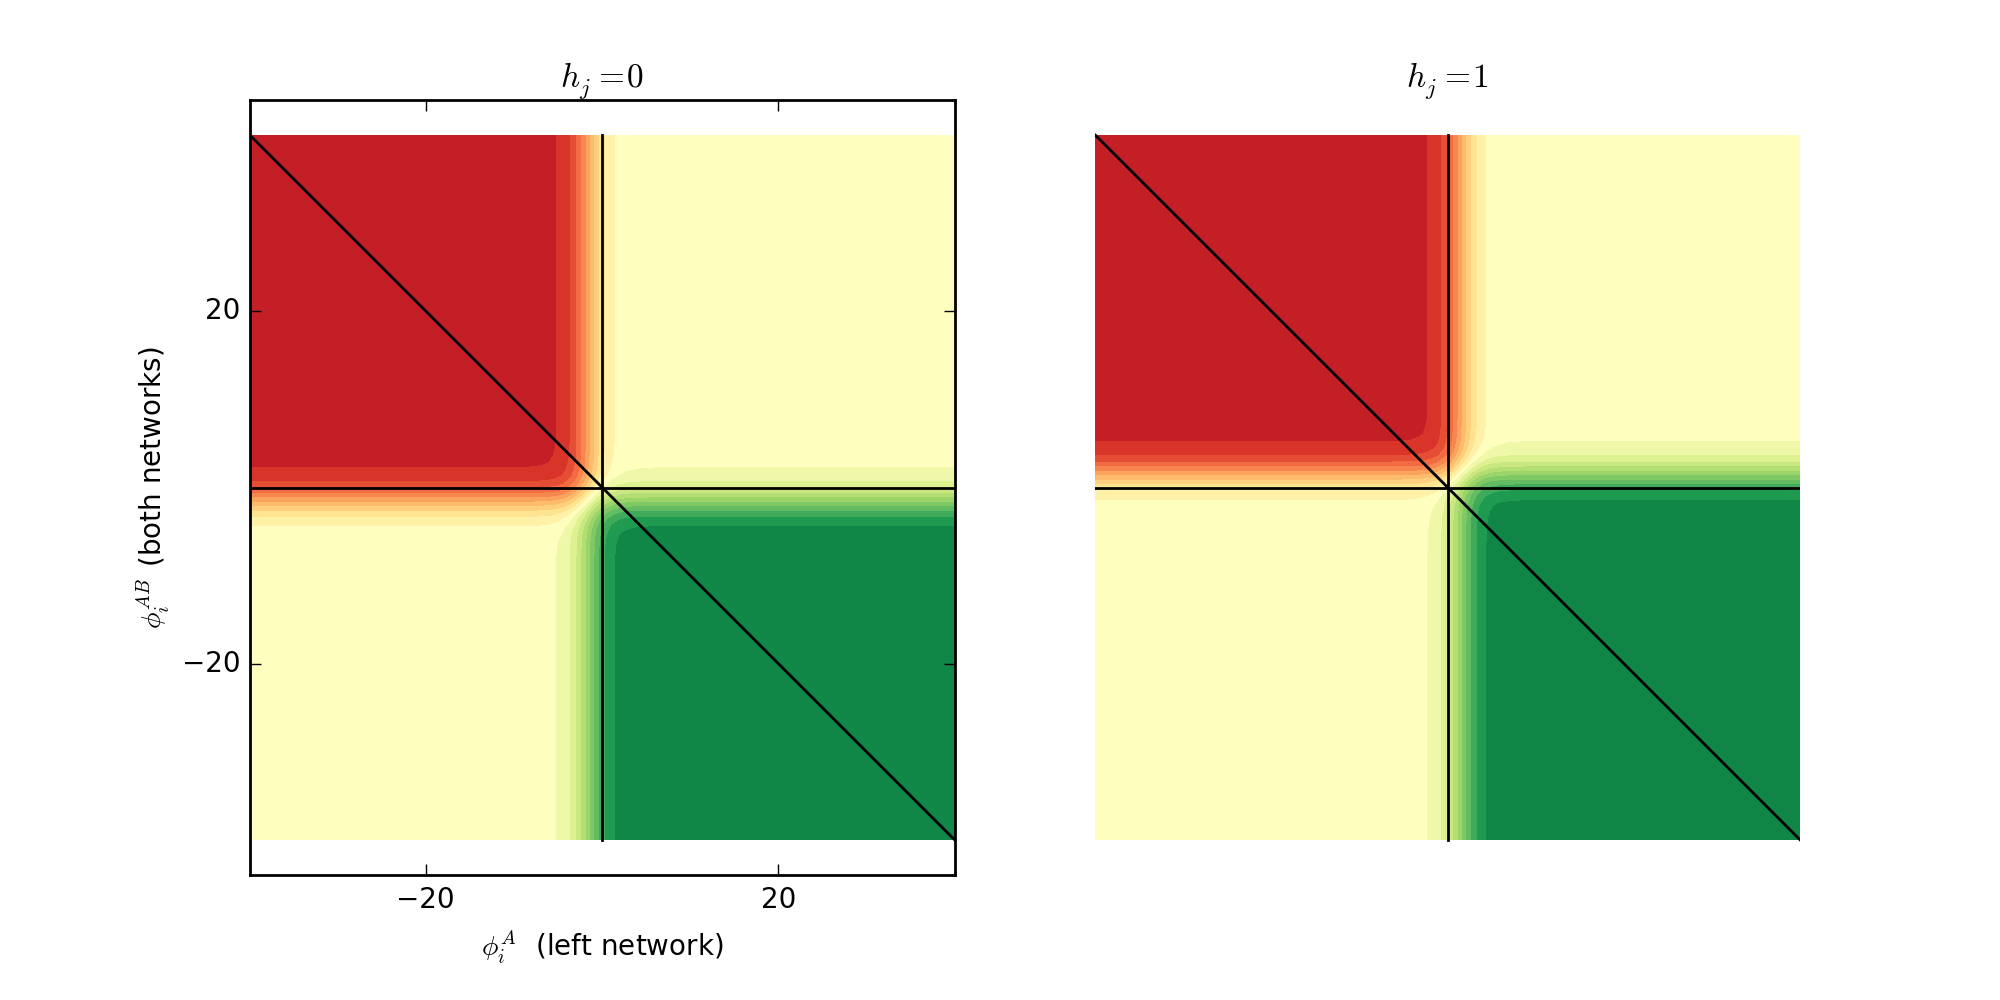
\includegraphics[width = 0.8\textwidth]{Assets/correction.png}
\caption{A diagram that shows the structure of the correction over the weighted sums into the hiddens of one of the RBMS versus both. Note the platuaes that are $+- weight$ in maganitude}
\label{F:Correction-Plot}
\end{center}
\end{figure}

\subsubsection{What happened to the biases?}

The ORBM utilises the hidden biases present on the RBMs when calculating the hidden states $h^A$ and $h^B$. However, the visible biases are not used in sampling from the visible. The reasoning behind this being that the RBMs visible bias acts like the `background rate`, i.e. what visible reconstruction would we see from an all zero hidden activation. As visible bias are not captured in the ORBM, it is important that RBMs plugged into it's structure do not use a visible bias.

\subsubsection{Reconstructions and Dreams in the ORBM}

Reconstructions in the ORBM are a natural extension of the inference algorithm.
\begin{itemize}
  \item First hidden representations $h^A$ and $ h^B $ are generated given an input $v$.
  \item The RBMs (RBM A and B) uses their respective hidden representations to generate visible patterns independently. That is, we can use the same way of performing Gibbs sampling we saw in equation \ref{eq:Vis-Gibbs-Update}.
\end{itemize}
This means that for a visible pattern there are potentially two reconstructions, one from each model.
